%!TEX TS-program = xelatex
%!TEX encoding = UTF-8 Unicode
%!TEX backend = biblatex


\documentclass[10pt,twocolumn,letterpaper]{article}

\usepackage{cvpr}
\usepackage{times}
\usepackage{epsfig}
\usepackage{graphicx}
\usepackage{amsmath}
\usepackage{amssymb}
\usepackage{fontspec,xltxtra,xunicode}
\bibliographystyle{unsrt}
\defaultfontfeatures{Mapping=tex-text}
%\setromanfont[Mapping=tex-text]{NSimSun}
\setsansfont[Scale=MatchLowercase,Mapping=tex-text]{Hiragino Sans GB}
\usepackage{xeCJK}
\renewcommand{\baselinestretch}{1.4}
\renewcommand\figurename{图}
%\XeTeXlinebreaklocale "zh"
%\XeTeXlinebreakskip = 0pt plus 1pt

%\setmonofont[Scale=MatchLowercase]{Andale Mono}

% Include other packages here, before hyperref.

% If you comment hyperref and then uncomment it, you should delete
% egpaper.aux before re-running latex.  (Or just hit 'q' on the first latex
% run, let it finish, and you should be clear).
\usepackage[breaklinks=true,bookmarks=false]{hyperref}

\cvprfinalcopy % *** Uncomment this line for the final submission

\def\cvprPaperID{****} % *** Enter the CVPR Paper ID here
\def\httilde{\mbox{\tt\raisebox{-.5ex}{\symbol{126}}}}

% Pages are numbered in submission mode, and unnumbered in camera-ready
%\ifcvprfinal\pagestyle{empty}\fi
\setcounter{page}{1}
\begin{document}

%%%%%%%%% TITLE
\title{深度学习在物体检测与识别中的应用}

\author{熊郁文\\
3130000829\\
{\tt\small orpine@zju.edu.cn}
% For a paper whose authors are all at the same institution,
% omit the following lines up until the closing ``}''.
% Additional authors and addresses can be added with ``\and'',
% just like the second author.
% To save space, use either the email address or home page, not both
%\and
%Second Author\\
%Institution2\\
%First line of institution2 address\\
%{\tt\small secondauthor@i2.org}
}

\maketitle
%\thispagestyle{empty}

%%%%%%%%% ABSTRACT
\begin{abstract}
在大规模图像数据中进行精确的物体检测与识别是计算机视觉中一个非常重要的问题。从2012年以来,深度学习在图像分类问题方面取得了令人瞩目的成绩。而在物体检测方面,自2014年开始,Ross Girshick在CVPR 2014上发表的论文中提出了R-CNN,成功的将深度学习应用到物体检测中,并取得了远好于传统方法的结果。本文将对2014年以来,使用卷积神经网络在物体检测问题上取得良好结果的算法进行简要介绍,包括R-CNN~\cite{girshick14CVPR},SPP-net~\cite{he2014spatial},Fast R-CNN~\cite{girshickICCV15fastrcnn}以及Faster R-CNN~\cite{ren2015faster}。
\end{abstract}

%%%%%%%%% BODY TEXT
\section{引言}
物体的检测一直是计算机视觉中比较重要和困难的问题。在很多领域有广泛的应用,比如安保方面的的行人检测与跟踪,交通领域的车辆检测等等。因此这个问题在计算机视觉,模式识别与机器学习等领域都是非常活跃的研究方向。传统的方法一直是基于SIFT或者HOG等手工设计的特征,在此基础上进行一些工作。然而这些方法已经被证实效果并不理想,SegDPM~\cite{fidler2013bottom}在Pascal VOC 2010数据集上的表现也仅有40.4\%的mAP,远远称不上令人满意。卷积神经网络(CNN)是由20世纪80年代由Yann LeCun提出的一种神经网络,最初用于手写数字识别~\cite{lecun1989backpropagation},其特殊的结构使其对二维的图像数据输入能得到非常好的结果。但由于当时的机器性能限制,CNN未能得到更多的关注。直到2012年,Geoffrey Hinton的博士生Alex Krizhevsky利用一个8层的CNN在ILSVRC 2012的图像分类任务上一举取得了远超以往算法的成绩~\cite{krizhevsky2012imagenet}。点燃了学术界对于深度卷积神经网络在计算机视觉方面的研究的热情,但在当时,深度卷积神经网络只在一定程度上解决了对整张图像的分类问题,而更加困难的对图片中多个物体进行定位与识别的问题还尚未解决。本文将对深度卷积神经网络在物体检测与识别方面的研究进展做简要介绍。第二节将介绍将卷积神经网络拓展到物体检测问题上并在PASCAL VOC竞赛中取得突破性进展的的第一种方法——R-CNN,R-CNN证明了CNN提取出来的『Rich feature』效果远远好于传统的方法,第三节将介绍在R-CNN基础上进行改进,去除了R-CNN的冗余计算使得速度与效果都得到提升的SPP-net与Fast R-CNN,第四节将介绍R-CNN的最新进展——Faster R-CNN,这种算法进一步提升了Fast R-CNN的速度,基本能够做到实时的物体检测。文章的最后将对这几种算法做一个总结,并对未来进行展望。

\section{R-CNN介绍}
R-CNN由Ross Girshick等人于CVPR 2014上提出。在这之前,大家已经意识到CNN在图像分类方面的威力,而如何才能将CNN应用在物体检测方面这是一个问题。与图像分类问题不同之处在于,物体的检测问题需要定位出物体的位置。R-CNN将Pipeline分为三部分来解决用CNN进行物体检测的问题。第一个部分试图生成与待检测的物体类别无关(category-independent)的region proposal,有别于传统的sliding window做法,这些region proposal就是检测目标的“候选”,后续的检测识别将只会在这些region proposal上进行。第二部分是用于提取图像特征的深度卷积神经网络。第三部分则是一组用来对CNN提取出的特征进行类别分类的线性SVM。这样就成功的将物体检测问题变成了在bounding box中的图像分类问题。
\begin{figure}[htbp] %  figure placement: here, top, bottom, or page
   \centering
   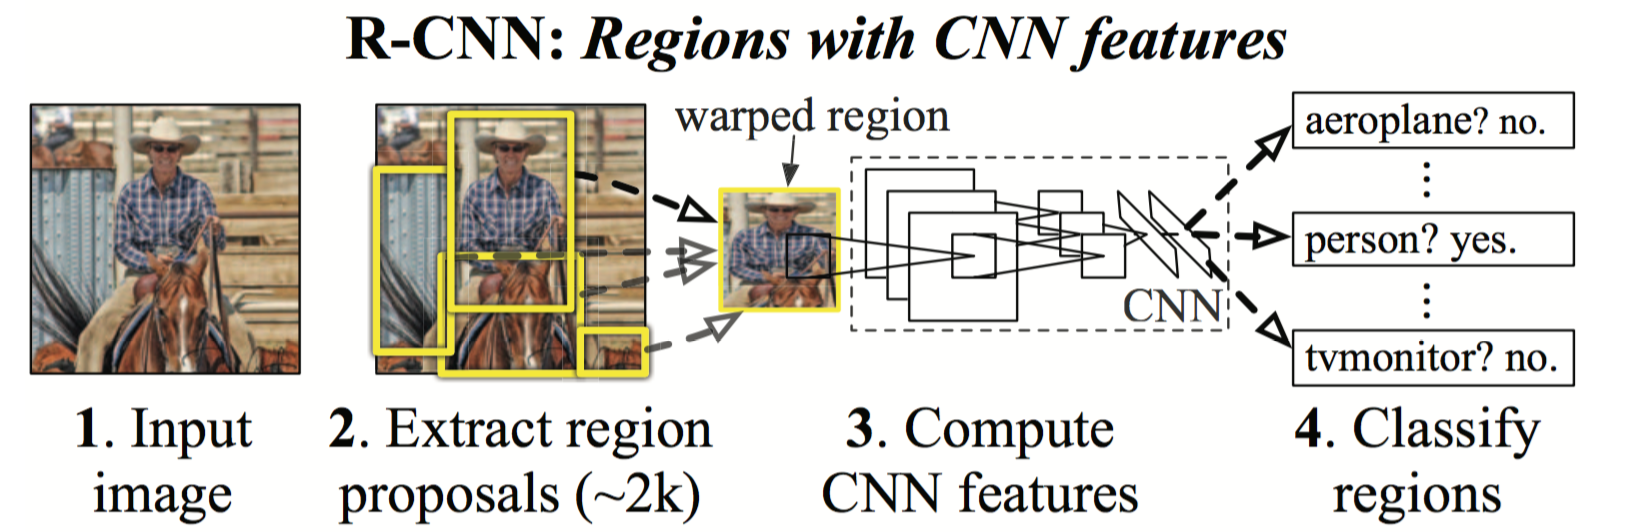
\includegraphics[width=3in]{rcnn.png} 
   \caption{R-CNN 框架图}
   \label{figure:rcnn}
\end{figure}
\subsection{R-CNN设计}
第一个问题是,如何快速的得到region proposal,得益于前人的工作,我们有许多现成的方法可以使用,包括objectness,selective search,category-independent object proposals,constrained parametric min-cuts (CPMC),multi-scale combinatorial grouping等等。作者在R-CNN中使用的是selective search。

作者使用了Alex Krizhevsky在ILSVRC 2012中所使用的CNN网络AlexNet~\cite{krizhevsky2012imagenet},对于每个输入,去掉最后一层softmax分类层而提取出了一个4096维的特征向量。需要注意的是,对于AlexNet这样有全连接层的网络,输入图片的大小是有严格限制的(作者使用的网络版本是227x227) ,因此对于每个region proposal,作者使用了wrapping的方式即将每个region proposal缩放成规定大小的正方形来作为输入。

最后,基于时间和内存的考量,作者选择了线性SVM作为最后的分类器。

\subsection{R-CNN的训练与测试}

作者提出,可以将利用ILSVRC 2012年数据训练的AlexNet作为一个提取图片的特征的黑盒,但是为了让处理分类问题的网络在处理物体识别问题上也工作的很好,我们需要对其进行fine-tuning。在Fine-tuning阶段,作者在AlexNet权值的基础上,将最后一层1000路Softmax改为了PASCAL VOC所需的21类,对于selective search获取的region proposal,与ground-truth bounding box的IoU $\geqslant 0.5$的region proposal被认为是positive sample,否则是背景。

之后,利用Fine-tuning过后的CNN来提取特征(提取出Softmax层之前的4096位向量),利用提取出来的特征来训练SVM,作者对每一类检测物体训练一个SVM。在训练中,作者将与任意ground-truth bounding box的IoU(Intersection of Union)$\geqslant 0.5$的region proposal认为是正样本,与所有ground-truth bounding box的 $\leqslant 0.3$ 的region proposal认为是负样本,其余丢弃。作者指出在这里通过验证集选择一个合适的阈值是十分重要的,对mAP结果会有较大的影响。同时,由于内存问题,作者对于SVM采用了hard negative mining的训练方法,不过考虑到这不是本文介绍重点,而且作者在后续文章中放弃了SVM作为分类器,在此就不再赘述了。

在测试时,对于每一张输入图片,作者会使用selective search来提取两千个左右的region proposal,wrap后将其送入CNN中提取出feature,再利用SVM来进行分类确定每个region proposal的类别(是否为某一类物体或者是背景)。最后再利用non-maximum suppression去除掉重叠的bounding box。

作者另外还实现了bounding box regression,这在本文以及后续文章的实验中被证实是一种十分有效的减少mislocation的做法,通过训练数据(ground truth中标记的位置与feature vector)训练出一个线性回归模型,试图对selective search所找到的region proposal的位置进行修正(输出bounding box中心点以及长、宽的修正量),这种做法对mAP能有3-4\%的提升,具体的转换可在作者主页上的supplement中找到。
\subsection{R-CNN的总结}
R-CNN被认为是CNN在物体检测领域的开山之作。而且它让人们意识到特征在计算机视觉领域的重要性,这也从论文标题看得出来,标题并没有强调『R-CNN』这一方法,而是强调『Rich feature hierarchies』。
在测试结果上,R-CNN相较于以往的方法确实有相当大的提高(在PASCAL VOC 2010数据集上mAP从40.4\%提升至53.7\%),但其对于数据处理过于粗糙,仍有提升的空间(后面将介绍的几种方法也证实了这一点)。对于每张输入图片,selective search都会提取出1\~{}2千个不等的region proposal要通过CNN进行feature提取,这些region proposal有许多是互相重叠的,因此有大量冗余的计算,这也导致了R-CNN的速度非常之慢,提取出来的feature也要暂存到硬盘上,中间文件可能会有上百GB之多,这都是R-CNN的缺陷。

\section{SPP-net与Fast R-CNN介绍}
SPP-net由Kaiming He等人于ECCV 2014上提出。Fast R-CNN则由Ross Girshick自己在ICCV 2015上提出,鉴于他们俩较为相似,这里将它们放在一起介绍。

SPP-net是基于R-CNN所做的一些改进,Fast R-CNN是在SPP-net上进一步改进之后的结果。相比SPP-net有更快的速度与更好的结果。接下来将主要介绍他们与R-CNN所不同的部分。

\subsection{SPP-net的改进}
Kaiming He等人首先注意到了R-CNN的不足之处——第一,由于CNN的全连接层对feature vector的长度有要求,对于不满足指定大小的region proposal,无论是warpping或是cropping的做法,都会在一定程度上损失原有数据的信息,不利于正确识别图像;第二,对于同一张图片,region proposal有上千个,其中很多都是重叠的,会有大量的重复计算。

值得一提的是,CNN中的卷积层对于输入实际上是没有任何约束的,也就是说卷积层可以处理任意尺度的输入,是之后的全连接层限制了这一点。因此,为了解决这个问题,Kaiming He等人在R-CNN中引入了空间金字塔池化(Spatial Pyramid Pooling (SPP) layer)。其本质就是,对于一个feature map做多个尺度的池化。由图\ref{figure:sppnet}中可以看到,对于从AlexNet的第五层卷积层输出的feature map,对它们做1x1,2x2,4x4的池化,由于conv5有256个filter,所以最后的结果会是一个256维的向量、4个256维的向量和16个256维的向量。最后将他们连接起来成为全连接层的输入。此时我们可以发现,这种处理方式对于图片的大小是没有要求的,因为中间这一层池化,对于任意尺度的图片都可以处理成定长的feature vector(图中所给的例子是(1+4+16)X256=5376维)然后在输入给全连接层。
\begin{figure}[htbp] %  figure placement: here, top, bottom, or page
   \centering
   \includegraphics[width=3in]{sppnet.png} 
   \caption{SPP layer 结构}
   \label{figure:sppnet}
\end{figure}

SPP layer的引入,成功解决了第一个问题。在test阶段,对于selective search得到的region proposal,如何不进行feature map的重复计算?我们现在已经有能力直接对整张图片计算feature map,那么实际上就可以通过计算直接将region proposal在原图片中的位置转换为在conv5输出的feature map中的位置(这一步转换公式较为复杂)。这样一来原本较为耗时的CNN的计算就转变成了四个坐标值的计算,大大减少了计算时间。在文章中作者将原始图片放大成若干大小,选取region proposal在缩放后的图像中大小最接近224x224的图片。最后的时间消耗上相对于R-CNN有数十倍的提升(在PASCAL VOC 2007的测试集上单张图片0.382s vs 14.46s)。

\subsection{Fast R-CNN的改进}

Fast R-CNN一文指出R-CNN有三个明显的缺陷:第一,训练时pipeline被分为了三个阶段,对于使用selective search提取好的region proposal,需要先利用CNN提取特征,然后再训练分类器(R-CNN与SPP-net都使用了SVM),最后训练bounding box regression,十分麻烦和复杂。也因此导致了空间开销十分之大,这里是可以考虑进行简化的;第二,训练时太耗时间和内存及硬盘空间;第三,测试阶段速度太慢。而SPP-net在加速了R-CNN的同时,并没有解决第一个缺陷,同时还引入了别的问题:无法更新SPP layer之前的网络层的权值,对于更深的网络来说,这样将会限制网络的精度。

而Fast R-CNN则将训练的三个阶段统一起来,提高速度的同时也去除了额外磁盘空间的限制。大致框架如图\ref{figure:frcn}。
\begin{figure}[htbp] %  figure placement: here, top, bottom, or page
   \centering
   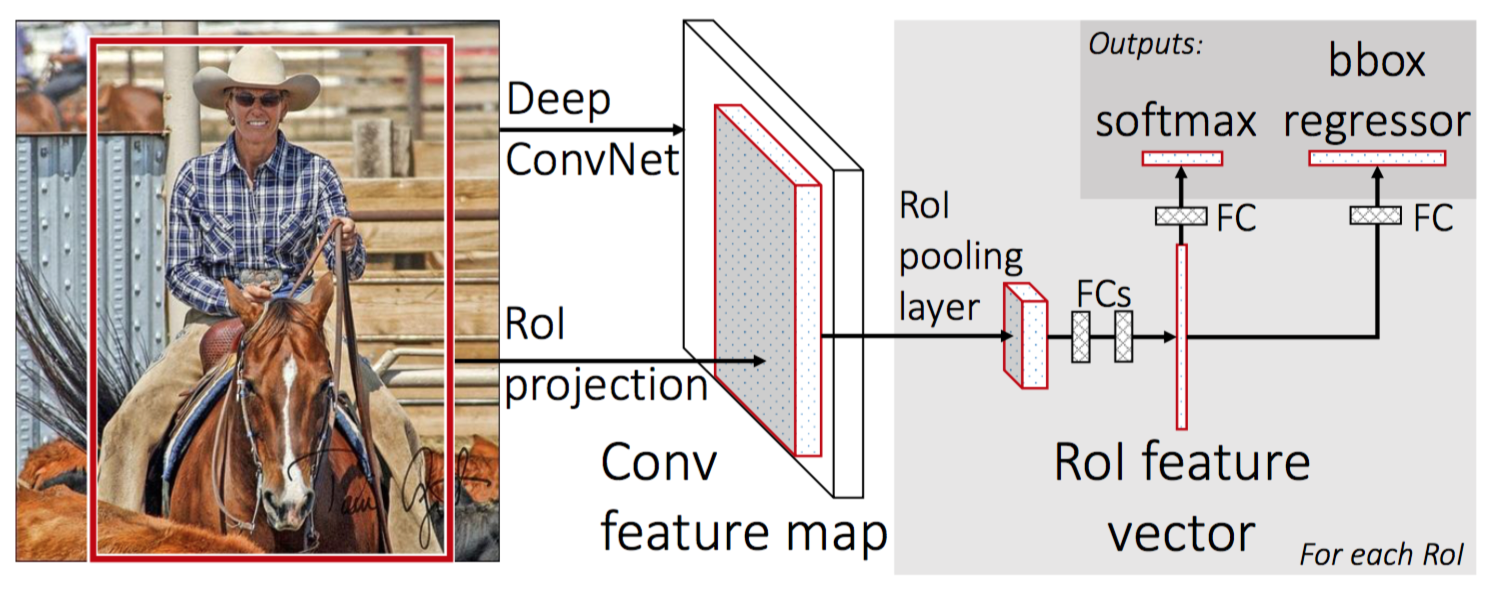
\includegraphics[width=3in]{frcn.png} 
   \caption{Fast R-CNN 结构}
   \label{figure:frcn}
\end{figure}

作者在文章中提出了RoI pooling layer,这实际上是SPP layer layer的一种简化版本,模仿SPP layer,我们可以将任意大小的图片max pooling成 $H\times W$ 的大小(文章中为$7\times 7$),而RoI pooling layer的意义在于,对于提取到一半的feature map,给定一个region proposal,我们可以算出它在feature map中的位置,并通过RoI pooling 得到一个固定大小的feature map如$7\times 7$将其送入后续的layer,同时RoI pooling layer也可以进行反向传导,更新RoI pooling layer前面的网络层权值。这样一来,CNN只需处理每张图片一次,再利用RoI pooling layer处理每个region proposal即可。同时作者指出R-CNN和SPP-net 在fine-tuning时效率是十分低下的,原因是训练样本都是来自许多不同的图片,这样会导致训练的输入太大。而Fast R-CNN每次只使用两张图片,每张图片提取64个region proposal来构成一个大小为128的mini-batch。由于一张图片只需要过一次CNN,这种方式会比R-CNN中对于每个region proposal都需要warpping并且过一遍CNN的做法速度大大提升。

Fast R-CNN还将分类器替换为softmax,并把它与bounding box regressor统一起来同时进行joint traning,提出了smooth-L1作为bounding box regression的loss function,认为这种函数形式将会提高鲁棒性,在全连接层还利用了SVD分解来减少需要训练的参数进行加速。而在测试时,之前所描述的SPP-net会对图像进行多个尺度的缩放然后从缩放的图片中选取大小合适的region proposal,而Fast R-CNN则采取了将所有图片缩放到一个固定尺度的做法。前者比后者可以比后者得到稍好一点的结果(mAP增加1\%左右),但后者的速度会快很多,而且对于规模更大的网络(如VGG16),现有GPU的12G显存限制无法做到多尺度的缩放。

Fast R-CNN在网络上做得多处改进使得其比SPP-net又快上数倍(在PASCAL VOC 2007的测试集上单张图片0.32s vs 2.3s),在PASCAL VOC 2007上的mAP也达到了68.8\%。

作者同时还在文章中给出一些其他的insight,如更多的data将会带来更好的结果,region proposal的数量需要正好合适而不是越多越好等等,这对我们更加深入的理解物体检测领域的一些细节有所帮助,但不是本文介绍重点。

\section{Faster R-CNN介绍}
Faster R-CNN是Kaiming He等人与Ross Girshick合作在微软研究院所做的工作。在NIPS 2015上发表。

Fast R-CNN成功的将CNN,classifier与bounding box regressor统一,这三部分都利用了GPU加速运行,此时利用selective search提取region proposal的部分就变成了瓶颈,因为这部分是跑在CPU上的。能否将提取region proposal的工作也转移到GPU上运行,将整个框架统一起来做到真正的end-to-end呢?答案是肯定的,这就是Faster R-CNN主要所做的工作,通过定义一种新的网络结构,Faster R-CNN做到了又快又好的提取region proposal。

为了让region proposal的提取也能在GPU上运行,作者提出了一种叫做Region Proposal Networks(RPN)的网络结构。这是一个全部由卷积层构成的网络,作者在实验中使用了ZF model~\cite{Zeiler:2014fr}的前5层和VGG~\cite{Simonyan14c}的前13层 。作者指出,对于卷积网络输出的feature map,也可以用于提取region proposal。作者在feature map上使用了一个小型的网络进行滑动窗口的扫描。提取出一个低维向量(对于ZF和VGG两种不同规模的网络,长度分别为256和512)。最后将这个向量送入两个全连接层。这一部分如图\ref{fig:rpn}所示
\begin{figure}[htbp] %  figure placement: here, top, bottom, or page
   \centering
   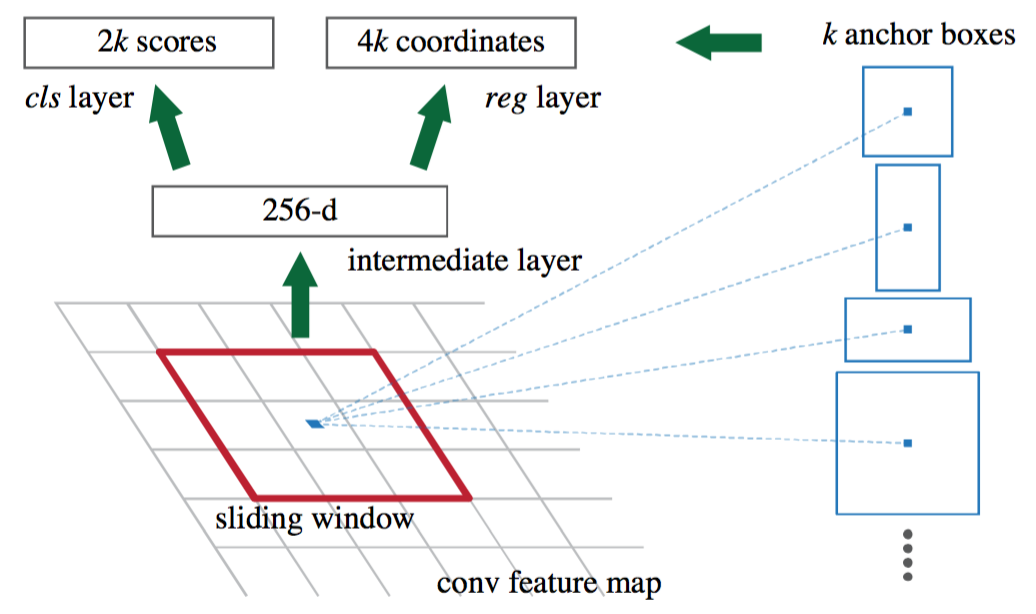
\includegraphics[width=3in]{rpn.png} 
   \caption{RPN结构}
   \label{fig:rpn}
\end{figure}
对于每个窗口,作者进行了多个尺度与高宽比的采样,生成k个anchor(对于从窗口中采样得到的region proposal,作者在论文中称为anchor),文中使用了三种尺度与三种高宽比,最后对于每个窗口将会产生9个anchors,因此k=9。在训练时,作者将与某个ground-truth box的IoU>0.7的anchor标记为positive,与所有的groun-truth box的IoU都<0.3的anchor标记为negative,其余的anchor以及超过了图片边界的anchor将被丢弃。RPN最后的两个全连接层cls layer与reg layer分别会产生2k个score(为了实现上的方便,作者采用了2类的softmax层来给出第k个anchor是物体/背景的判断)以及4k个coordinates(即第k个anchor的bounding box regression结果)。值得注意的是,Fast R-CNN对于任意大小的region proposal都是用相同的bounding box regressor,而此处有k个regressor对应不同大小的anchor。

为了做到图片在网络中的『1-pass』,作者还将RPN与后面处理anchor的Fast R-CNN的卷积层进行了权值共享,同时进一步降低参数个数,加快速度,提高鲁棒性。这里有很多种做法,作者在论文中提出了一种『4步做法』,先独立训练一个RPN,将得到的anchor送入Fast R-CNN中训练Fast R-CNN,再利用Fast R-CNN的网络参数初始化RPN,固定卷积层参数微调RPN的全连接层。最后再微调Fast R-CNN的全连接层。这样一来,两部分网络共享了卷积层的参数,而又有各自不同的全连接层参数。之后,作者更在GitHub的开源代码中给出了end-to-end的训练方式,这种方式简化了训练步骤,同时效果并未减弱。

因为RPN可以利用GPU进行加速,Faster R-CNN的速度又上升了一个台阶。将selective search替换为RPN后,耗费时间可以达到原来的1/10,在作者的实验中,使用VGG + Fast R-CNN时每秒可处理五张图片。换成规模小一点的ZF网络则每秒可以处理17张图片,已经达到距离实时处理仅有一步之遥。


\section{总结}
本文简要介绍了近两年来物体检测领域的主流算法,鉴于篇幅原因,有许多细节未能详细介绍,如果感兴趣的话可以去查阅相关论文。从14年Ross Girshick提出R-CNN到如今,也才不过短短两年多的时间,计算机视觉在物体检测领域的进展可用突飞猛进来形容。从R-CNN一路走来,SPP-net,Fast R-CNN,Faster R-CNN。速度越来越快,检测精度越来越高,让我们又一次感受到了深度学习的能力,同时Kaiming He等人也从别的角度入手,在2015年提出Deep Residual Network,将CNN网络提升至前所未有的152层~\cite{He2015},今年更是加深到1000层以上~\cite{He2016}。利用更好的feature配合Faster R-CNN取得了ILSVRC 2015年的图像检测任务冠军。同时Ross Girshick在Fast R-CNN工作中所做的实验也发现,对于深度学习来说,增加数据对mAP的提升仍有帮助,让我们不禁细想深度学习的极限在何处。在PASCAL VOC数据集上,mAP从40\%到50\%到60\%再到70\%,速度也从非实时做到了准实时,接下来的提升可能会越来越困难,从R-CNN一脉相承的这一套方法仍然存在一个缺陷,那就是没有用到图片中的context信息来获取先验知识,如果能够整合这一点,想必又能做到一个提升,我们期望在不久的将来能看到mAP提升到95\%甚至更高的那天。




%-------------------------------------------------------------------------
%\subsection{语言}
%
%All manuscripts must be in English.
%
%\subsection{Dual submission}
%
%Please refer to the author guidelines on the CVPR 2015 web page for a
%discussion of the policy on dual submissions.
%
%\subsection{Paper length}
%For CVPR 2015, the rules about paper length have changed, so please
%read this section carefully. Papers, excluding the references section,
%must be no longer than eight pages in length. The references section
%will not be included in the page count, and there is no limit on the
%length of the references section. For example, a paper of eight pages
%with two pages of references would have a total length of 10 pages.
%{\bf Unlike previous years, there will be no extra page charges for
%  CVPR 2015.}
%
%Overlength papers will simply not be reviewed.  This includes papers
%where the margins and formatting are deemed to have been significantly
%altered from those laid down by this style guide.  Note that this
%\LaTeX\ guide already sets figure captions and references in a smaller font.
%The reason such papers will not be reviewed is that there is no provision for
%supervised revisions of manuscripts.  The reviewing process cannot determine
%the suitability of the paper for presentation in eight pages if it is
%reviewed in eleven.  
%
%%-------------------------------------------------------------------------
%\subsection{The ruler}
%The \LaTeX\ style defines a printed ruler which should be present in the
%version submitted for review.  The ruler is provided in order that
%reviewers may comment on particular lines in the paper without
%circumlocution.  If you are preparing a document using a non-\LaTeX\
%document preparation system, please arrange for an equivalent ruler to
%appear on the final output pages.  The presence or absence of the ruler
%should not change the appearance of any other content on the page.  The
%camera ready copy should not contain a ruler. (\LaTeX\ users may uncomment
%the \verb'\cvprfinalcopy' command in the document preamble.)  Reviewers:
%note that the ruler measurements do not align well with lines in the paper
%--- this turns out to be very difficult to do well when the paper contains
%many figures and equations, and, when done, looks ugly.  Just use fractional
%references (e.g.\ this line is $095.5$), although in most cases one would
%expect that the approximate location will be adequate.
%
%\subsection{Mathematics}
%
%Please number all of your sections and displayed equations.  It is
%important for readers to be able to refer to any particular equation.  Just
%because you didn't refer to it in the text doesn't mean some future reader
%might not need to refer to it.  It is cumbersome to have to use
%circumlocutions like ``the equation second from the top of page 3 column
%1''.  (Note that the ruler will not be present in the final copy, so is not
%an alternative to equation numbers).  All authors will benefit from reading
%Mermin's description of how to write mathematics:
%\url{http://www.pamitc.org/documents/mermin.pdf}.
%
%
%\subsection{Blind review}
%
%Many authors misunderstand the concept of anonymizing for blind
%review.  Blind review does not mean that one must remove
%citations to one's own work---in fact it is often impossible to
%review a paper unless the previous citations are known and
%available.
%
%Blind review means that you do not use the words ``my'' or ``our''
%when citing previous work.  That is all.  (But see below for
%techreports.)
%
%Saying ``this builds on the work of Lucy Smith [1]'' does not say
%that you are Lucy Smith; it says that you are building on her
%work.  If you are Smith and Jones, do not say ``as we show in
%[7]'', say ``as Smith and Jones show in [7]'' and at the end of the
%paper, include reference 7 as you would any other cited work.
%
%An example of a bad paper just asking to be rejected:
%\begin{quote}
%\begin{center}
%    An analysis of the frobnicatable foo filter.
%\end{center}
%
%   In this paper we present a performance analysis of our
%   previous paper [1], and show it to be inferior to all
%   previously known methods.  Why the previous paper was
%   accepted without this analysis is beyond me.
%
%   [1] Removed for blind review
%\end{quote}
%
%
%An example of an acceptable paper:
%
%\begin{quote}
%\begin{center}
%     An analysis of the frobnicatable foo filter.
%\end{center}
%
%   In this paper we present a performance analysis of the
%   paper of Smith \etal [1], and show it to be inferior to
%   all previously known methods.  Why the previous paper
%   was accepted without this analysis is beyond me.
%
%   [1] Smith, L and Jones, C. ``The frobnicatable foo
%   filter, a fundamental contribution to human knowledge''.
%   Nature 381(12), 1-213.
%\end{quote}
%
%If you are making a submission to another conference at the same time,
%which covers similar or overlapping material, you may need to refer to that
%submission in order to explain the differences, just as you would if you
%had previously published related work.  In such cases, include the
%anonymized parallel submission~\cite{Authors14} as additional material and
%cite it as
%\begin{quote}
%[1] Authors. ``The frobnicatable foo filter'', F\&G 2014 Submission ID 324,
%Supplied as additional material {\tt fg324.pdf}.
%\end{quote}
%
%Finally, you may feel you need to tell the reader that more details can be
%found elsewhere, and refer them to a technical report.  For conference
%submissions, the paper must stand on its own, and not {\em require} the
%reviewer to go to a techreport for further details.  Thus, you may say in
%the body of the paper ``further details may be found
%in~\cite{Authors14b}''.  Then submit the techreport as additional material.
%Again, you may not assume the reviewers will read this material. 
%
%Sometimes your paper is about a problem which you tested using a tool which
%is widely known to be restricted to a single institution.  For example,
%let's say it's 1969, you have solved a key problem on the Apollo lander,
%and you believe that the CVPR70 audience would like to hear about your
%solution.  The work is a development of your celebrated 1968 paper entitled
%``Zero-g frobnication: How being the only people in the world with access to
%the Apollo lander source code makes us a wow at parties'', by Zeus \etal.
%
%You can handle this paper like any other.  Don't write ``We show how to
%improve our previous work [Anonymous, 1968].  This time we tested the
%algorithm on a lunar lander [name of lander removed for blind review]''.
%That would be silly, and would immediately identify the authors. Instead
%write the following:
%\begin{quotation}
%\noindent
%   We describe a system for zero-g frobnication.  This
%   system is new because it handles the following cases:
%   A, B.  Previous systems [Zeus et al. 1968] didn't
%   handle case B properly.  Ours handles it by including
%   a foo term in the bar integral.
%
%   ...
%
%   The proposed system was integrated with the Apollo
%   lunar lander, and went all the way to the moon, don't
%   you know.  It displayed the following behaviours
%   which show how well we solved cases A and B: ...
%\end{quotation}
%As you can see, the above text follows standard scientific convention,
%reads better than the first version, and does not explicitly name you as
%the authors.  A reviewer might think it likely that the new paper was
%written by Zeus \etal, but cannot make any decision based on that guess.
%He or she would have to be sure that no other authors could have been
%contracted to solve problem B.
%
%FAQ: Are acknowledgements OK?  No.  Leave them for the final copy.
%
%
%\begin{figure}[t]
%\begin{center}
%\fbox{\rule{0pt}{2in} \rule{0.9\linewidth}{0pt}}
%   %\includegraphics[width=0.8\linewidth]{egfigure.eps}
%\end{center}
%   \caption{Example of caption.  It is set in Roman so that mathematics
%   (always set in Roman: $B \sin A = A \sin B$) may be included without an
%   ugly clash.}
%\label{fig:long}
%\label{fig:onecol}
%\end{figure}
%
%\subsection{Miscellaneous}
%
%\noindent
%Compare the following:\\
%\begin{tabular}{ll}
% \verb'$conf_a$' &  $conf_a$ \\
% \verb'$\mathit{conf}_a$' & $\mathit{conf}_a$
%\end{tabular}\\
%See The \TeX book, p165.
%
%The space after \eg, meaning ``for example'', should not be a
%sentence-ending space. So \eg is correct, {\em e.g.} is not.  The provided
%\verb'\eg' macro takes care of this.
%
%When citing a multi-author paper, you may save space by using ``et alia'',
%shortened to ``\etal'' (not ``{\em et.\ al.}'' as ``{\em et}'' is a complete word.)
%However, use it only when there are three or more authors.  Thus, the
%following is correct: ``
%   Frobnication has been trendy lately.
%   It was introduced by Alpher~\cite{Alpher02}, and subsequently developed by
%   Alpher and Fotheringham-Smythe~\cite{Alpher03}, and Alpher \etal~\cite{Alpher04}.''
%
%This is incorrect: ``... subsequently developed by Alpher \etal~\cite{Alpher03} ...''
%because reference~\cite{Alpher03} has just two authors.  If you use the
%\verb'\etal' macro provided, then you need not worry about double periods
%when used at the end of a sentence as in Alpher \etal.
%
%For this citation style, keep multiple citations in numerical (not
%chronological) order, so prefer \cite{Alpher03,Alpher02,Authors14} to
%\cite{Alpher02,Alpher03,Authors14}.
%
%
%\begin{figure*}
%\begin{center}
%\fbox{\rule{0pt}{2in} \rule{.9\linewidth}{0pt}}
%\end{center}
%   \caption{Example of a short caption, which should be centered.}
%\label{fig:short}
%\end{figure*}
%
%%------------------------------------------------------------------------
%\section{Formatting your paper}
%
%All text must be in a two-column format. The total allowable width of the
%text area is $6\frac78$ inches (17.5 cm) wide by $8\frac78$ inches (22.54
%cm) high. Columns are to be $3\frac14$ inches (8.25 cm) wide, with a
%$\frac{5}{16}$ inch (0.8 cm) space between them. The main title (on the
%first page) should begin 1.0 inch (2.54 cm) from the top edge of the
%page. The second and following pages should begin 1.0 inch (2.54 cm) from
%the top edge. On all pages, the bottom margin should be 1-1/8 inches (2.86
%cm) from the bottom edge of the page for $8.5 \times 11$-inch paper; for A4
%paper, approximately 1-5/8 inches (4.13 cm) from the bottom edge of the
%page.
%
%%-------------------------------------------------------------------------
%\subsection{Margins and page numbering}
%
%All printed material, including text, illustrations, and charts, must be kept
%within a print area 6-7/8 inches (17.5 cm) wide by 8-7/8 inches (22.54 cm)
%high.
%Page numbers should be in footer with page numbers, centered and .75
%inches from the bottom of the page and make it start at the correct page
%number rather than the 4321 in the example.  To do this fine the line (around
%line 23)
%\begin{verbatim}
%%\ifcvprfinal\pagestyle{empty}\fi
%\setcounter{page}{4321}
%\end{verbatim}
%where the number 4321 is your assigned starting page.
%
%Make sure the first page is numbered by commenting out the first page being
%empty on line 46
%\begin{verbatim}
%%\thispagestyle{empty}
%\end{verbatim}
%
%
%%-------------------------------------------------------------------------
%\subsection{Type-style and fonts}
%
%Wherever Times is specified, Times Roman may also be used. If neither is
%available on your word processor, please use the font closest in
%appearance to Times to which you have access.
%
%MAIN TITLE. Center the title 1-3/8 inches (3.49 cm) from the top edge of
%the first page. The title should be in Times 14-point, boldface type.
%Capitalize the first letter of nouns, pronouns, verbs, adjectives, and
%adverbs; do not capitalize articles, coordinate conjunctions, or
%prepositions (unless the title begins with such a word). Leave two blank
%lines after the title.
%
%AUTHOR NAME(s) and AFFILIATION(s) are to be centered beneath the title
%and printed in Times 12-point, non-boldface type. This information is to
%be followed by two blank lines.
%
%The ABSTRACT and MAIN TEXT are to be in a two-column format.
%
%MAIN TEXT. Type main text in 10-point Times, single-spaced. Do NOT use
%double-spacing. All paragraphs should be indented 1 pica (approx. 1/6
%inch or 0.422 cm). Make sure your text is fully justified---that is,
%flush left and flush right. Please do not place any additional blank
%lines between paragraphs.
%
%Figure and table captions should be 9-point Roman type as in
%Figures~\ref{fig:onecol} and~\ref{fig:short}.  Short captions should be centred.
%
%\noindent Callouts should be 9-point Helvetica, non-boldface type.
%Initially capitalize only the first word of section titles and first-,
%second-, and third-order headings.
%
%FIRST-ORDER HEADINGS. (For example, {\large \bf 1. Introduction})
%should be Times 12-point boldface, initially capitalized, flush left,
%with one blank line before, and one blank line after.
%
%SECOND-ORDER HEADINGS. (For example, { \bf 1.1. Database elements})
%should be Times 11-point boldface, initially capitalized, flush left,
%with one blank line before, and one after. If you require a third-order
%heading (we discourage it), use 10-point Times, boldface, initially
%capitalized, flush left, preceded by one blank line, followed by a period
%and your text on the same line.
%
%%-------------------------------------------------------------------------
%\subsection{Footnotes}
%
%Please use footnotes\footnote {This is what a footnote looks like.  It
%often distracts the reader from the main flow of the argument.} sparingly.
%Indeed, try to avoid footnotes altogether and include necessary peripheral
%observations in
%the text (within parentheses, if you prefer, as in this sentence).  If you
%wish to use a footnote, place it at the bottom of the column on the page on
%which it is referenced. Use Times 8-point type, single-spaced.
%
%
%%-------------------------------------------------------------------------
%\subsection{References}
%
%List and number all bibliographical references in 9-point Times,
%single-spaced, at the end of your paper. When referenced in the text,
%enclose the citation number in square brackets, for
%example~\cite{Authors14}.  Where appropriate, include the name(s) of
%editors of referenced books.
%
%\begin{table}
%\begin{center}
%\begin{tabular}{|l|c|}
%\hline
%Method & Frobnability \\
%\hline\hline
%Theirs & Frumpy \\
%Yours & Frobbly \\
%Ours & Makes one's heart Frob\\
%\hline
%\end{tabular}
%\end{center}
%\caption{Results.   Ours is better.}
%\end{table}
%
%%-------------------------------------------------------------------------
%\subsection{Illustrations, graphs, and photographs}
%
%All graphics should be centered.  Please ensure that any point you wish to
%make is resolvable in a printed copy of the paper.  Resize fonts in figures
%to match the font in the body text, and choose line widths which render
%effectively in print.  Many readers (and reviewers), even of an electronic
%copy, will choose to print your paper in order to read it.  You cannot
%insist that they do otherwise, and therefore must not assume that they can
%zoom in to see tiny details on a graphic.
%
%When placing figures in \LaTeX, it's almost always best to use
%\verb+\includegraphics+, and to specify the  figure width as a multiple of
%the line width as in the example below
%{\small\begin{verbatim}
%   \usepackage[dvips]{graphicx} ...
%   \includegraphics[width=0.8\linewidth]
%                   {myfile.eps}
%\end{verbatim}
%}
%
%
%%-------------------------------------------------------------------------
%\subsection{Color}
%
%Please refer to the author guidelines on the CVPR 2015 web page for a discussion
%of the use of color in your document.
%
%%------------------------------------------------------------------------
%\section{Final copy}
%
%You must include your signed IEEE copyright release form when you submit
%your finished paper. We MUST have this form before your paper can be
%published in the proceedings.
%

{\small
\bibliographystyle{ieee}
\bibliography{egbib}
}

\end{document}
